%%%%%%%%%%%%%%%%%%%%%%%%%%%%%%%%%%%%%%%%%
% University/School Laboratory Report
% LaTeX Template
% Version 3.1 (25/3/14)
%
% This template has been downloaded from:
% http://www.LaTeXTemplates.com
%
% Original author:
% Linux and Unix Users Group at Virginia Tech Wiki 
% (https://vtluug.org/wiki/Example_LaTeX_chem_lab_report)
%
% License:
% CC BY-NC-SA 3.0 (http://creativecommons.org/licenses/by-nc-sa/3.0/)
%
%%%%%%%%%%%%%%%%%%%%%%%%%%%%%%%%%%%%%%%%%

%----------------------------------------------------------------------------------------
%	PACKAGES AND DOCUMENT CONFIGURATIONS
%----------------------------------------------------------------------------------------

\documentclass{article}

\usepackage[margin=1in]{geometry}
\usepackage{amsmath} % Required for some math elements 
\usepackage{enumitem}
\usepackage{graphicx}
\usepackage{subcaption}

\setlength\parindent{0pt} % Removes all indentation from paragraphs

\newlist{inlinelist}{enumerate*}{1} %code to allow inline numbering of items
\setlist*[inlinelist,1]{%
  label=(\arabic*),
}

%\renewcommand{\labelenumi}{\alph{enumi}.} % Make numbering in the enumerate environment by letter rather than number (e.g. section 6)

%\usepackage{times} % Uncomment to use the Times New Roman font

%----------------------------------------------------------------------------------------
%	DOCUMENT INFORMATION
%----------------------------------------------------------------------------------------

\title{\begin{LARGE}
	\textbf{EE 445L - Lab 2: Performance Debugging}
\end{LARGE}} % Title

\author{Joshua Bryant \\ jmb6357 \and James Morris \\ jsm3288} % Author name

\date{\today} % Date for the report

\begin{document}

\maketitle % Insert the title, author and date

%----------------------------------------------------------------------------------------
%	SECTION 1 Objectives
%----------------------------------------------------------------------------------------

\section{Objective} %simply copied from Goals section in lab doc
 The five main objectives for this lab are: 
 \begin{inlinelist}
 	\item developing software debugging techniques
 	\item passing data using a FIFO queue
 	\item learning how to use the oscilloscope and logic analyzer
 	\item observing critical sections, and
 	\item getting an early start on Lab 3 by writing a line drawing function
 \end{inlinelist}. The specific software debugging techniques used for this lab include performance debugging in real time and profiling program activity.
 
%----------------------------------------------------------------------------------------
%	SECTION 2 Hardware Design
%----------------------------------------------------------------------------------------

%\section{Hardware Design} %not needed for this lab.

%----------------------------------------------------------------------------------------
%	SECTION 3 Software Design
%----------------------------------------------------------------------------------------

%\section{Software Design} %not needed for this lab. Just upload files to Canvas

%----------------------------------------------------------------------------------------
%	SECTION 4 Measurement Data
%----------------------------------------------------------------------------------------

\section{Measurement Data} %Mostly screenshots from the o-scopes in the lab, get these from James
	\subsection{Part B and C}
		\centering		
		\begin{figure}[h]
			\centering
			\begin{subfigure}{0.45\textwidth}
				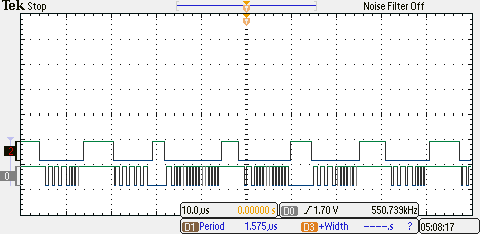
\includegraphics[keepaspectratio, width=\textwidth]{Lab2Screens/Lab2PartB1.png}
				\caption{Part B screen shot}
				\label{fig:SS_B}
			\end{subfigure}
			\hfill
			\begin{subfigure}{0.45\textwidth}
				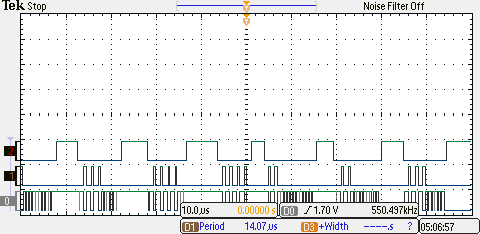
\includegraphics[keepaspectratio, width=\textwidth]{Lab2Screens/Lab2PartC5}	
				\caption{Part C screen shot}
				\label{fig:SS_C}
			\end{subfigure}
			\caption{In both images, line 2 shows the interrupt occurring with two successive interrupts}
			\label{fig:SS_B&C}			
			\hfill		
		\end{figure}
		\raggedright		
		
	\subsection{Part E}
		\centering
		\begin{figure}[h]
			\centering
			\begin{subfigure}{0.45\textwidth}
				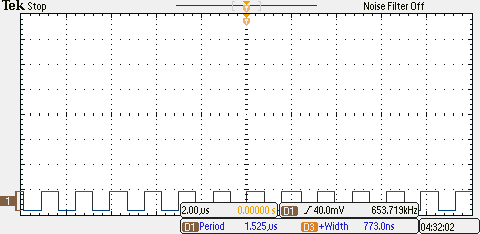
\includegraphics[keepaspectratio, width=\textwidth]{Lab2Screens/Lab2PartE1}
				\caption{Execution time of RxFifo\_Get}
				\label{fig:SS_E1}
			\end{subfigure}
			\hfill
			\begin{subfigure}{0.45\textwidth}
				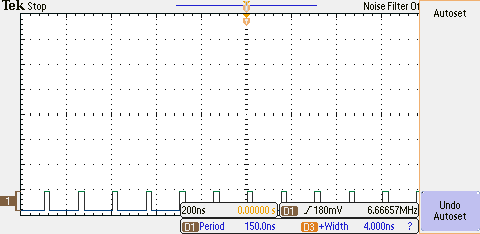
\includegraphics[keepaspectratio, width=\textwidth]{Lab2Screens/Lab2PartE2}
				\caption{Execution time of toggling pins}
				\label{fig:SS_E2}
			\end{subfigure}
			\label{fig:SS_E}
			\hfill
		\end{figure}
		\raggedright
		The SysTick technique had the benefit of providing not only the execution time of each cycle of RxFifo\_Get but also additional data that can be useful when trying to debug issues with code. This comes at the expense of being, at best, minimally intrusive. The scope technique has the advantage of being less intrusive to the program than the SysTick techniques but its downside is not providing as much data for use in debugging code.
		
	\subsection{Part H}
		\centering
		\begin{figure}[h]
			\centering
			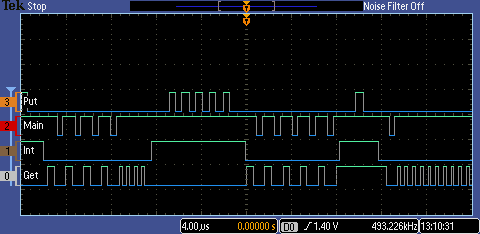
\includegraphics[keepaspectratio, width=0.6\textwidth]{Lab2Screens/Lab2PartH}
			\caption{Screen shot of oscilloscope showing two interrupts}
		\end{figure}
		\raggedright
%----------------------------------------------------------------------------------------
%	SECTION 5 Analysis and Discussion
%----------------------------------------------------------------------------------------

\section{Analysis and Discussion}

\begin{enumerate}
	\item %Question 1
		We did not measure the same result for execution speed of RxFifo\_Get for all three methods. The first method of printing out the cycle count after returning from RxFifo\_Get was the least intrusive but only stored one value from FIFO at a time and wrote over it every execution. Using printf inside the RxFifo\_Get function was the most intrusive but had the benefit of providing not only the execution time but also the data received from the FIFO and the current FIFO pointer for ever execution cycle. The memory dump provided only the the first 10 data values recieved from the FIFO but was less intrusive than inserting the printf function into RxFifo\_Get leading to a value generally between the values measured by the original FIFO function and the FIFO function with printf inside.

	\item %Question 2
		If you expected the execution speed to vary a lot, you should use the data dump technique. This technique is less intrusive than printing data to a screen and the amount of time needed to dump data each execution cycle should remain almost constant. This technique also allows for storing a large number of data entries for review later to allow averaging over hundreds of samples for average execution time as well as finding the most likely minimum and maximum execution times.

	\item %Question 3
		If the expected execution speed is very large, using printf output is appropriate provided small strings were used for output. Although printf can be very intrusive in faster programs, the long execution period means that outputing a few characters won't significantly slow down the program, as discussed in class.

	\item %Question 4
		Minimally intrusive debugging techniques are defined to have a negligible effect on the system being debugged.

	\item %Question 5
		The two necessary components collected during a "profile" are the timing characteristics and the execution patterns of a program.

	\item %Question 6
		The critical sections in the bad FIFO were at the increment and decrement since they happen after the value being changed is called from memory but before it is being stored. The way to fix this problem on ARM would be to include the post-increment and post-decrement inside the functions using these values as parameters. This is clear after viewing both the standard FIFO and bad FIFO code side by side.

\end{enumerate}

\end{document}